%!TEX root = ../masters_thesis.tex

\chapter{Development} % (fold)
\label{cha:development}

The aim of this thesis is to create a Historical Geographic Information System to visualize and edit the evolution of countries in time and space. This is a complicated task, because both the reality and the human that should be able to use the system are complex. The task is to create an interface that a human can easily understand and use. For complex applications in which the interface matters, the methodologies of \emph{Human Centered Design} are promising to achieve a good solution.

The development process is iterative divided in several phases. In each phase, the fidelty towards the final solution is increased. A phase starts with an initial set of requirements about the problem. In multiple iterations, an interface is developed that solves the problem. Each iteration has four steps: The requirements for the system are analyzed in the \emph{planning} step. Afterwards, they translated into an abstract \emph{design} which is realized in a specific \emph{implementation} of the interface. Finally, this interface is tested with humans to find out how well it works. Based on the results of this \emph{testing} step, the requirements are updated and the next iteration starts. This is repeated until a version of the interface is created that sufficiently solves the problem. Then the fidelity is increased, starting the next development phase.

The five phases in this thesis were:
\begin{compactenum}
  \item \textbf{Idea}: The initial idea how to edit and visualize the history of countries.
  \item \textbf{Paper Prototype}: The concept of the interface realized and tested on paper.
  \item \textbf{Mockup Prototype}: The concrete workflow developed in a slide-based presentation.
  \item \textbf{Web-Based Prototype}: The final version developed in a Web application.
  \item \textbf{Extensions}: Design approaches how to fit the uncertain nature of history.
\end{compactenum}

\begin{figure}[H]
  \centering
  \includegraphics[width=0.8\textwidth]{graphics/development/hcd}
  \caption{Human Centered Design process with five project phases}
  \label{fig:hcd}
\end{figure}

There are several models involved in the development of the software, each of them has to be developed or analyzed separately. The \emph{data model} is an abstraction and simplification of the real world. The \emph{Hivent Model} created in this thesis is explained in the first section \ref{sec:hivent_model} of this chapter. In iteractive computer systems, the \emph{mental model} is the representation in the mind of the human about how the interface he or she is interacting with should work. On the other hand, the \emph{conceptual model} describes the way the interface actually works. The goal of Human Centered Design is to match the conceptual model to the mental model. Section \ref{sec:histoglobe_interface} outlines the gradual interface design process to reach this goal. In the application, the implemented \emph{database model} has to match the abstract data model. The task for the \emph{computational model} is to translate between the database model and the conceptual model. The working of the HistoGlobe application, including the computational model, is introduced in the last section \ref{sec:histoglobe_application} of this chapter.

\begin{figure}[H]
  \vspace{1em}
  \centering
  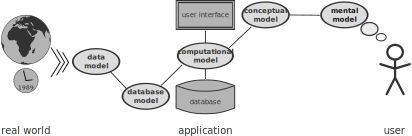
\includegraphics[width=0.8\textwidth]{graphics/development/models}
  \caption{Relevant models for the system}
  \label{fig:models}
\end{figure}

% ==============================================================================
\section{Hivent Model} % (fold)
\label{sec:hivent_model}

This section introduces the data model that represents countries and their evolution in time and space. In section \ref{sec:spatio_temporal_data_models}, different spatio-temporal data models were introduced to solve this problem. The \emph{Snapshot Model} is unsuitable for the problem space. \emph{Simple Time-Stamping} is helpful to link countries to their history, but it does not explicitly model historical changes, which is desireable. For that purpose, the idea of the \emph{Event-Based Spatio-Temporal Data Model} was developed, but since it only works for raster data, it is also not suitable for this thesis. This problem is solved in the \emph{History Graph Model}. Additionally, the introduced temporal changes allow to represent historical changes and their influences on geographic entities directly in the model. Finally, the \emph{Three-Domain Model} introduces a helpful concept to separate the spatial, temporal and thematic dimension of a spatio-temporal entity.

The \emph{Hivent Model} is constructed from components of some of these models: An Event-Based Spatio-Temporal Data Model supporting vector data. It is organized according to the Three-Domain Model, uses Simple Time-Stamping to define the lifetime of a spatial entity, and to visualize it on a History Graph. In the first section of this section, the main elements of the Hivent model are introduced. Afterwards, the preconditions are defined. Finally, the Historical Geographic Operations that describe changes of countries in time and space are explained.

% ------------------------------------------------------------------------------
\subsection{Elements} % (fold)
\label{sub:elements}

The main elements of the the model are \emph{Hivent}s, representing an historically significant happening and \emph{Area}s, an abstract entity on a map with a name and a territory. An \emph{Historical Change} is part of one Hivent and manipulates the history of one or more Areas.

% - - - - - - - - - - - - - - - - - - - - - - - - - - - - - - - - - - - - - - -
\vspace{-1em}
\paragraph{Hivents} % (fold)
\label{par:hivent}

are the main organizing elements of the data model. The word is an acronym for \emph{\textbf{Hi}}storical e\emph{\textbf{vent}}. It represents a significant happening in history, e.g. a treaty, bill or declaration. The focus in this work is on events that influence the geopolitical situation on Earth. An Hivent happens at one particular point in time and space and introduces historical changes to countries.

% paragraph hivent (end)

% - - - - - - - - - - - - - - - - - - - - - - - - - - - - - - - - - - - - - - -
\vspace{-1em}
\paragraph{Areas} % (fold)
\label{par:area}

represent one identical current or historical country with a \emph{name} and a \emph{territory} on the map. The name of the Area consists of a common \emph{short name}, e.g. ``Germany'' and a \emph{formal name}, e.g. ``Federal Republic of Germany''. The \emph{territory} of the Area is described by a polypolygon, a set of weakly simple polygons to support enclaves and exclaves. The polylines of the polygons consist of an ordered set of points that represent the country border. The borders of a country are either \emph{interior}, i.e. bordering another country, or a \emph{coastline}, bordering a body of water.

% paragraph area (end)

% ------------------------------------------------------------------------------
\vspace{-1em}
\paragraph{Historical Changes} % (fold)
\label{par:historical_changes}

influence the development of an Area over time. Throughout the lifetime of an Area, it is created at some point $t_s$, then its territory and short name can change multiple times $t_i: t_s < t_i$ and at some point $t_e: t_s < t_i < t_e$ it ceases. Since all changes in this model are sudden, there are only two possible states an Area can be in: It is \emph{active}, if at the current time point it is historically existing and it is \emph{inactive} if it does not. Each area is uniquely identified by its formal name. That means, the short name can change, but as soon as the formal name of an area changes (e.g. ``German Empire'' to ``Federal Republic of Germany''), it is considered a ``new'' Area.

Each Historical Change belongs to exactly one Hivent, inheriting its time point at which the change happens.  The change is described by a Historical Geographic Operation introduced in section \ref{sub:historical_geographic_operations}.

\begin{figure}[H]
  \vspace{1em}
  \centering
  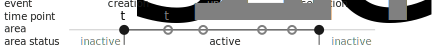
\includegraphics[width=0.9\textwidth]{graphics/development/area_states}
  \caption{Three event types that change Areas, resulting in two different area states}
  \label{fig:area_states}
\end{figure}


% paragraph historical_changes (end)

% subsection section area (end)

% ------------------------------------------------------------------------------
\subsection{Preconditions} % (fold)
\label{sub:preconditions}

\begin{quoteit}
In the beginning God created the heavens and the Earth \\
Now the Earth was formless and empty [...] \\
And God said, “Let there be light” --- and there was light.
\end{quoteit}
\hfill -- Genesis 1:1, The First Book of Moses, Old Testament

There are five axoims and two assumptions that are the basis of the spatio-temporal system developed in this thesis. The theoretical foundation is the model of the Earth, its curved surface that can be projected on a two-dimensional map using a map projection, as introduced in sections \ref{sub:model_of_geographical_space} and \ref{sub:presentation_of_geographic_space}.

\vspace{-1.0em}
\newtheorem{invariant_surface}[assicounter]{Axiom}
\begin{invariant_surface}
\label{axm:invariant_surface}
  The Earth's surface has an invariant area size, i.e. it does not change over time.
\end{invariant_surface}

\vspace{-2.5em}
\newtheorem{area_on_surface}[assicounter]{Axiom}
\begin{area_on_surface}
\label{axm:area_on_surface}
  Each Area in the spatio-temporal system is located directly on the surface of the Earth.
\end{area_on_surface}

These axiom sets the spatial foundation of the system: a constant dimension of the map and Areas covering the map. The basis of the temporal part of the system is content of the next three axioms:

\vspace{-1.0em}
\newtheorem{initial_configuration}[assicounter]{Axiom}
\begin{initial_configuration}
\label{axm:initial_configuration}
  The spatio-temporal system has an initial state at time point $t_0$. At this initial state, there exists exactly one Area, denoted by $\Omega$ and referred to as the \emph{universe} Area. It has no name and its territory covers the whole surface of the Earth.
\end{initial_configuration}

\vspace{-2.5em}
\newtheorem{historical_change}[assicounter]{Axiom}
\begin{historical_change}
\label{axm:historical_change}
  At each time point $t_i \geq t_0$ an Historical Change can be introduced.
\end{historical_change}

\vspace{-2.5em}
\newtheorem{unique_coverage}[assicounter]{Axiom}
\begin{unique_coverage}
\label{axm:unique_coverage}
  At each time point $t_i \geq t_0$ each point on the surface of the Earth is covered by exactly one territory of exactly one Area.
\end{unique_coverage}

As it has been defined in section \ref{par:historical_changes}, an Historical Change can create, manipulate and cease Areas on the Earth's surface. According to axoim \ref{axm:unique_coverage}, each change introduced in the system must maintain the spatial integrity on the map: When an Area with a territory is created on the map, the Area claiming this territory before has to cease this territory. Formally, it can be said that each change consists of a set of old Areas $A$ that are manipulated, a set of new Areas $B$ that are created in the change, and an operation $\rightarrow_C$ describing the change. Each Area $A_i \in A$ and $B_i \in B$ has a territory $A_i^T$  respectively $B_i^T$. For each change introduced in the system, the territories of the old Areas must have the same size than the territories of the new Areas to maintain the spatial integrity of axiom \ref{axm:unique_coverage}:
\begin{align}
  \bigcup\limits_{i=1}^n A_i^T ~\textbf{=}~ \bigcup\limits_{i=1}^n B_i^T
\end{align}

The first Historical Changes introduced in the system at time point $t_0$ are the creation of all bodies of water, including the oceans and lakes, denoted as $W$. Each Area $W_i \in W$ is created with their name and territory cut out of $\Omega$. The result is that at $t_0$, the map is divided into water ($W$) and land ($\Omega$). Land can at any point in time be either \emph{claimed}, i.e. it is currently occupied by the territory of exactly one active Area, or on a contrary be \emph{unclaimed}, i.e. belonging to $\Omega$. It is a subtractive data model, because each new Areas territory is cut out of $\Omega$.

\begin{figure}[H]
  \centering
  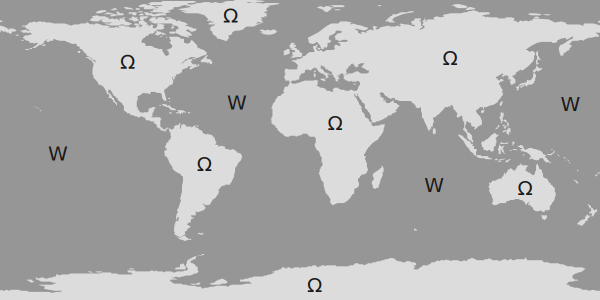
\includegraphics[width=0.5\textwidth]{graphics/development/init_map}
  \caption{The initial state of the world map at time point $t_0$}
  \label{fig:init_map}
\end{figure}

In the real world, the name of a country changes according to sudden events, e.g. a declaration or a governmental bill. The territory can change either because of a geographical processes, e.g. the sea level rise influencing the change of the coastline, or according to a historical event, e.g. a treaty. The Hivent model is based on two assumptions that simplify the model and keep the problem space clear:

\vspace{-1.0em}
\newtheorem{coastline_territory}[assicounter]{Assumption}
\begin{coastline_territory}
\label{axm:coastline_territory}
  The territory of a country stops at the coastline.
\end{coastline_territory}

\vspace{-1.5em}
\newtheorem{constant_coastlines}[assicounter]{Assumption}
\begin{constant_coastlines}
\label{axm:constant_coastlines}
  The spatial configuration of the Earth's surface, i.e. land, water and the coastlines, has not changed over time.
\end{constant_coastlines}

Both assumptions are obviously wrong: In line with \cite{UNSeaBorders}, the territory of a country extends in a range of 3 to 12 miles (5 to 20 kilometers) into international waters. They are constantly changing and so does the distribution of land and water on Earth. However, the assumptions allow the Hivent Model to focus only on discrete historical changes and not on long-term processes. In this data model, the temporal behavior of an Area can therefore be described as a \emph{static object that changes according to sudden events}.

% base: Newtons concept of absolute space?
% TODO: topological rule?
% each border has exactly two neighboring Areas
% each Area has at least one neighboring Area

% subsection preconditions (end)

% ------------------------------------------------------------------------------
\subsection{Historical Geographic Operations} % (fold)
\label{sub:historical_geographic_operations}

Respecting the preconditions, there are several different types of changes that can occur to a set of Areas. All possible changes can be expressed with only five spatio-temporal operations that are called \emph{Historical Geographic Operations} (HG Operations). The first four change the identity of a set of Areas and therefore establish historical predecessor-successor-relationships. They are always symmetric, i.e. if one old Area is replaced by one new Area, the old Area is the historical predecessor of the new Area and vice versa the new Area is the successor of the old Area.

\begin{description}
  \item[UNI -- Unification]
  A set of old Areas unifies to one new Area. The old Areas cease, becoming the historical predecessors of the new Area. This new Area receives a new name and its territory is the union of the territories of the old Areas. \\[0.25em]
  \begin{footnotesize}
    In 1922, the Russian SFSR, the Transcaucasian SFSR, the Ukrainian SSR and the Byelorussian SSR unified and formed the Union of Soviet Socialist Republics (USSR).
  \end{footnotesize}
  \item[INC -- Incorporation]
  One or more old Areas are incorporated into another Area that stays active. Its territory is enlarged by the union of the territories of the old Areas. The old Areas are historical predecessors of the new Area. \\[0.25em]
  \begin{footnotesize}
    In 1990, the territory of the German Democratic Republic (East Germany) became part of the Federal Republic of Germany (West Germany). Although this event is known as the \emph{German Reunification}, it is historically an incorporation of East Germany into West Germany \cite{incorporationEastWestGermany}.
  \end{footnotesize}
  \item[SEP -- Separation]
  As the inverse of unification, one old Area is preceded by multiple new Areas. Each new Area gets a new name, receives a part of the territory of the old Area, and the old Area as its only historical predecessor. \\[0.25em]
  \begin{footnotesize}
    In 1993, the Czech and Slovak Federal Republic, commonly known as Czechoslovakia, dissolved into present-day Czech Republic and Solvak Republic, creating two new countries out of one old.
  \end{footnotesize}
  \item[SEC -- Secession]
  As the inverse of incorporation, one or more new areas are ceded from a previously exising area that stays active. Each new Area gets a new name, receives the previously existing Area as the only historical predecessor and a part of its territory. \\[0.25em]
  \begin{footnotesize}
    In 2008, the Republic of Kosovo declared independence from Serbia and has since then partially received international recognition. Unlike in the case of separation, Serbia stays as country, keeping its name, but ceding a part of its territory to Kosovo.
  \end{footnotesize}
  \item[NCH -- Name Change]
  An Area changes its short name but preserves its identity. \\[0.25em]
  \begin{footnotesize}
    A recent change happened on 5. May 2016: The cabinet of Czech Republic approved that the country will now offically be called ``Czechia''. However, the formal name stays ``Czech Republic'', which preserves its identity.
  \end{footnotesize}
\end{description}

HG Operations can be combined when they happen at the same time, e.g. if one Area incorporates another Area and thereby changes its short name, this is a combination of \texttt{INC + NCH}. When West Germany incorporated East Germany in 1900, it was from that moment on just called Germany.

% - - - - - - - - - - - - - - - - - - - - - - - - - - - - - - - - - - - - - - -
\begin{table}[H]
\begin{center}
\begin{tabular}{m{0.75cm} m{2.5cm} m{2.5cm} m{2.0cm} m{2.5cm}}
  \toprule
  & operation
  & \multicolumn{1}{c}{visualization}
  & \multicolumn{1}{c}{\pbox{2.5cm}{historical\\relationship}}
  & \multicolumn{1}{c}{territory} \\

  \midrule
  \texttt{UNI} & Unification & \raisebox{-0.25\height}
  {
\includegraphics{graphics/development/hg_operations/UNI}} &
  $ A_i \leftrightarrow_H B_1 $ &
  $ B^T = \bigcup\limits_{i=1}^{n} A_i $ \\

  \midrule
  \texttt{INC} & Incorporation & \raisebox{-0.25\height}
  {\includegraphics{graphics/development/hg_operations/INC}} &
  $ A_i \leftrightarrow_H A_0 $ &
  $ A_0^T = \bigcup\limits_{i=1}^{n} A_i $ \\

  \midrule
  \texttt{SEP} & Separation & \raisebox{-0.25\height}
  {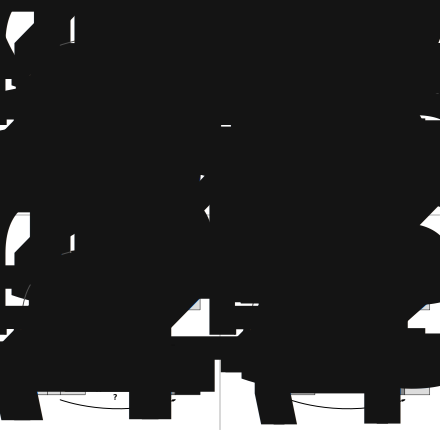
\includegraphics{graphics/development/hg_operations/SEP}} &
  $ A_1 \leftrightarrow_H B_i $ &
  $ B_i^T \cap A_1^T = B_i^T $ \\

  \midrule
  \texttt{SEC} & Secession & \raisebox{-0.25\height}
  {\includegraphics{graphics/development/hg_operations/SEC}} &
  $ A_0 \leftrightarrow_H B_i $ &
  $ B_i^T \cap A_0^T = B_i^T $ \\

  \midrule
  \texttt{NCH} & Name Change & \raisebox{-0.25\height}
  {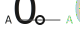
\includegraphics{graphics/development/hg_operations/NCH}} &
  $ \emptyset $ &
  $ \emptyset $ \\

  \bottomrule
\end{tabular}
\caption{Overview about the five HG Operations}
\small{$A_i \leftrightarrow_H B_i$ denotes: $\forall i \in [1..n]:$ $A_i$ is historical predecessor of $B_i$ and $B_i$ is successor of $A_i$}
\label{tab:historical_geographic_operations}
\end{center}
\end{table}

% subsection historical_geographic_operations (end)

% section hivent_model (end)

% ==============================================================================
\section{HistoGlobe Interface} % (fold)
\label{sec:histoglobe_interface}

The work of this thesis is developed in the HistoGlobe application. The Hivent Model shall be the basis of HistoGlobe. Developing the system bottom-up from the data model to the interface might lead to a system that is not well usable. Human Centered Design promotes a top-down process from the user via the interface into the core of the application. This process is introduced in this section. Figure \ref{fig:hcd} shows the five phases that lead from the identification of the mental model of the user all the way to the final interface and possible extensions to it that were not yet implemented.

The two main use cases for HistoGlobe that are focused in this thesis are:
\begin{compactenum}
  \item \textbf{Understanding} the history of countries.
  \item \textbf{Editing} the spatio-temporal evolution of countries with historical changes.
\end{compactenum}

For both use cases an appropriate visualization and interaction has to be designed. Throughout the development process, many interviews with historians and other researchers in humanities at University of Virginia were conducted to understand the mental model. The research confirmed that the combination of a map and a timeline are a very appropriate and intuitive way to interactively visualize the history of countries. Thefore, the main concept of HistoGlobe, introduced in section \ref{sec:histoglobe} does not need to be changed.

However, two extensions have emerged to be necessary modules: The \emph{HistoGraph} visualizes the history of countries aspatially on a graph. Its main idea is introduced in section \ref{sub:histograph}. Next to the normal exploration mode with map, timeline and HistoGraph, a need for an \emph{EditMode} to edit historical changes is proposed in section \ref{sub:editmode}. For editing purposes a different set of six \emph{EditOperations} were identified. The gradual process from the inital idea to the final user interface implemented in HistoGlobe is outlined in the last section \ref{sub:design_iterations}.

% ------------------------------------------------------------------------------
\subsection{HistoGraph} % (fold)
\label{sub:histograph}

Based on the idea of the History Graph Model (section \ref{fig:history_graph_model}), the linguistically and conceptually related \emph{HistoGraph} visualizes the history of countries on a graph. The edges of the graph represent an Area, the nodes an Hivent that changes the Areas evolution. The graph visualizes the historical predecessor-successor-relationships between Areas, a main feature of the Hivent Model. It allows to trace the evolution of the Area through time.

The two-dimensional HistoGraph has a horizontal orientation, expanding the timeline. The \texttt{x}-coordinate of the graph therefore refers to one time point on the timeline. The \texttt{y}-coordinate has no spatial or temporal relation. The graph uses the visualization approach of the five HG Operations (table \ref{tab:historical_geographic_operations}), including the following symbols (table \ref{tab:histograph_symbols}):

\begin{table}[H]
\begin{center}
\begin{tabular}{c l}

  \raisebox{3.5\height}
  {\includegraphics{graphics/development/histograph/line}}
  & Area \\

  \raisebox{-0.2\height}
  {
\includegraphics{graphics/development/histograph/circle_filled}}
  & Hivent with identity-changing HG Operation (\texttt{UNI}, \texttt{INC}, \texttt{SEP}, \texttt{SEC}) \\

  \raisebox{-0.2\height}
  {
\includegraphics{graphics/development/histograph/circle_unfilled}}
  & Hivent with property-changing HG Operation (\texttt{NCH}) \\

  \raisebox{-0.2\height}
  {
\includegraphics{graphics/development/histograph/circle_combo}}
  & Hivent with a combination of both (e.g. \texttt{INC + NCH} at the same time)

\end{tabular}
\caption{symbols used in the HistoGraph}
\label{tab:histograph_symbols}
\end{center}
\end{table}

The change resulting of an identity-changing HG Operation is visualized by a vertical line, indicating a sudden change with zero duration. From this line, the new Areas emerging from this change branch out right-angled. A horizontal line going straight through a circle indicates that the identity of the Area was preserved in the change. The HistoGraph is always created starting from one particular reference Area. It visualizes historically related Areas in one direction. That means, in historically backward direction, it recursively plots the predecessors and their predecessors on the graph, but not the predecessors successors. In the opposite historically forward direction, the successors and recursively the successors of the successors of the reference Area are plotted, but not their predecessors.

The behavior of the HistoGraph is shown for the example of the history of Germany since the end of World War II in figure \ref{fig:example_germany}. This history was driven by six historical events, which provide examples for all five HG Operations (table \ref{tab:german_history_since_1945}).

\begin{table}[H]
\begin{center}
\begin{tabular}{l p{8.5cm} l}
  \toprule
  Hivent date & Hivent description & HG Operations \\
  \midrule

    05.06.1945
  & \footnotesize{In the Berlin Declaration the total dissolution of the Third German Reich is confirmed. It separated into several different parts, returning the territories annexed by the German Reich in World War II to their original countries. The rest is controlled by the Allied Control Council in four occupation zones: the British, French, American and Soviet occupation zone.}
  & \texttt{SEP} \\

    16.02.1946
  & \footnotesize{The Saar Protectorate is entangled from the French Zone of Occupation Germany, creating an own country.}
  & \texttt{SEC} \\

    28.05.1949
  & \footnotesize{The Federal Republic of Germany (West Germany) is created from the British, American and French Zone of Occupation.}
  & \texttt{UNI} \\

    07.10.1949
  & \footnotesize{The German Democratic Republic (East Germany) is created from the Soviet Zone of Occupation}
  & \texttt{UNI} \\

    01.01.1957
  & \footnotesize{The Saar Treaty (``Little Reunification'') joins the Saar Protectorate as the Bundesland Saarland in West Germany.}
  & \texttt{INC} \\

    03.10.1990
  & \footnotesize{In the German Reunification, East Germany joins West Germany. The Federal Republic of Germany is now just called ``Germany''.}
  & \texttt{INC + NCH} \\

  \bottomrule
\end{tabular}
\caption{Historical events in German state history since 1945}
\label{tab:german_history_since_1945}
\end{center}
\end{table}

This example hosts a special case: in October 1949, East Germany was created from the Soviet Zone of occupation. Both Areas have the same territory, but a different short and formal name. A \texttt{NCH} can not be performed, because the identity is not preserved: The German Democratic Republic is a new Area. The change can be described by a \texttt{UNI} of only one Area (Soviet Zone), creating a new Area (East Germany) and establishing a historical relationship between both.

\begin{figure}[H]
  \vspace{1em}
  \centering
  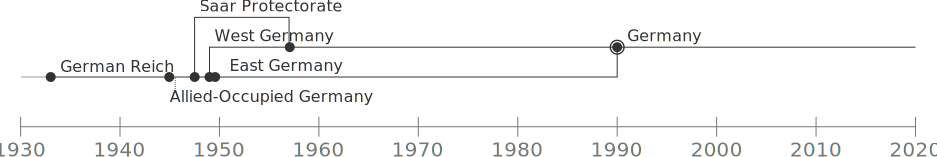
\includegraphics[width=0.8\textwidth]{graphics/development/histograph/example_germany}
  \caption{The concept of the HistoGraph at the example of the history of Germany since 1945}
  \label{fig:example_germany}
\end{figure}

The plot behavior becomes apparent in this example: starting from Germany, it plots East Germany as their predecessor incorporated in 1990. At the same date, it got renamed from West Germany to Germany, while still being the same Area. In 1957, the Saar Protectorate was incorporated. Its direct predecessor was the French Zone of Occupation. It is also one of the predecessors of West Germany, additional to the British and American Zone. East Germany was created from the Soviet Zone of Occupation. All of the four occupation zones originated from the German Reich. However, the German Reich dissolved into many more Areas, e.g. the Memel territory or the Polish Occupation Zone. They are not included in the graph, because they are not predecessors of any Area that is a recursive predecessor of present-day Germany.

This example also reveals many problems of the graph visualization: If many Hivents happened in a short period of time (in this case between 1945 and 1949), dots might overlap. Additionally, the names of the Areas of the four post-war occupation zones can not be shown in the Graph, because there is no space for them. The name ``West Germany'' collides with the vertical line indicating the incorporation of the Saar Protectorate, which should also be avoided. One more important aspect can be seen in the creation of West Germany in 1949: A \texttt{UNI} operation unifies three old Areas to one new Area. This could be visualized symmetrically with a straight line from the midmost incoming Area line into the Hivent circle to the outgoing Area line of the new Area. This would give the impression that this midmost Area has the same identity than the newly created Area, which is not the case. Therefore, the Hivent circle for \texttt{UNI} operations with an add number of old Areas must be displaced off the center, so that it becomes obvious that the identity has changed. All these issues are not in the scope of this thesis and subject to future work in the field of Information Visualization.

% subsection histograph (end)

% ------------------------------------------------------------------------------
\subsection{EditMode} % (fold)
\label{sub:editmode}

The user interface of HistoGlobe has two modi: The exploration mode to view the evollution of countries on a map with a timeline and a HistoGraph and the \emph{EditMode} proposed in this section. In the Human Centered Design process of this thesis, an interface was found that allows to intuitively edit historical changes directly in HistoGlobe, without the need to write data into database tables or standardised forms.

There two main use cases in the EditMode:
\begin{compactenum}
  \item Introduce an historical change to Areas on the map.
  \item Correcting the name or the territory of an Area on the map.
\end{compactenum}

Looking at the data model, both use cases lead to the same result: If the information at one point in history $t_1$ is wrong, e.g. the name of country $X$ should actually be $Y$, then this means the historical change that created name $X$ at time point $t_0$ is erroneous and has be changed. Especially if $t_0$ is far away in the past, the studies have shown that altering an historical change to correct an information on a map now is not very intuitive. Therefore, the EditMode is designed to do serve both use cases.

% - - - - - - - - - - - - - - - - - - - - - - - - - - - - - - - - - - - - - - -
\paragraph{EditOperations} % (fold)
\label{par:editoperations}

The question to be answered to introduce changes in the EditMode: What kind of changes can be introduced by a user that wants to edit the information about the evolution of countries in the system? Throughout the development process, many interviews with historians and other researchers in humanities at University of Virginia were conducted, to understand their mental model about historical changes of countries. Section \ref{sub:historical_geographic_operations} presented the five basic Historical Geographic Operations that can model all possible changes of countries in time and space. In the interviews it turned out that the HG Operations are not suitable to be used for human edit purposes, because of their low-level nature: The operations do not provide a straightforward way to create a new country on previously unclaimed land. Also changing the formal name of an Area is performed by a \texttt{UNI} operation, which is not very intuitive. The interviews revealed the following six high-level \emph{EditOperations} for introducing changes to countries on the map.

\begin{table}[H]
\begin{center}
\begin{tabular}{m{0.75cm} m{0.8cm} m{2.4cm} m{9.1cm}}
  \raisebox{-0.35\height}
  {
\includegraphics[width=0.75cm]{graphics/development/edit_operations/CRE}} &
  \texttt{CRE} & Create &
  a new Area with a new name and territory on the map. \\

  \raisebox{-0.35\height}
  {
\includegraphics[width=0.75cm]{graphics/development/edit_operations/MRG}} &
  \texttt{MRG} & Merge &
  two or more Areas to a new Area. The name has to be set manually, the territory is automatically unified. \\

  \raisebox{-0.35\height}
  {\includegraphics[width=0.75cm]{graphics/development/edit_operations/DIS}} &
  \texttt{DIS} & Dissolve &
  one Area into two or more new Areas, manually setting their new territory and name. \\

  \raisebox{-0.35\height}
  {
\includegraphics[width=0.75cm]{graphics/development/edit_operations/CHB}} &
  \texttt{CHB} & Change Borders &
  between two neighboring Areas by defining the territory that changes sides. \\

  \raisebox{-0.35\height}
  {\includegraphics[width=0.75cm]{graphics/development/edit_operations/REN}} &
  \texttt{REN} & Rename &
  an Area and set a new formal name, short name or both. \\

  \vspace{0.35em}
  \raisebox{-0.35\height}
  {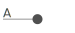
\includegraphics[width=0.75cm]{graphics/development/edit_operations/CES}} &
  \texttt{CES} & Cease &
  an Area by deleting it from the map, leaving unclaimed land. \\

\end{tabular}
\caption{Visualization of EditOperations}
\label{tab:hivent_to_hg_operations}
\end{center}
\end{table}

The EditOperations have proven to be understandable in several user studies in the development process of this thesis. The conceptual model will promote these six EditOperations that humans can understand, the data model is based on five related HG Operations that can model all cases of historical changes to countries in time and space. Therefore the task for the computational model of the HGIS is to translate between both operation sets.

% paragraph editoperations (end)

% - - - - - - - - - - - - - - - - - - - - - - - - - - - - - - - - - - - - - - -
\paragraph{Workflow} % (fold)
\label{par:workflow}

The idea of any of the six EditOperations is to introduce a change that transformes a set of old areas to a set of new areas. Therefore, the workflow consists of four EditOperation steps:

\begin{enumerate}
  \item \texttt{SELECT\_OLD\_AREAS}: The user selects the Areas that shall be manipulated by clicking them on the map.
  \item \texttt{CREATE\_NEW\_TERRITORIES}: For each Area that is to be created new in the step, the user creates a polypolygon describing the Areas territory either by clicking the territory manually or by importing it from an external source and then manipulating it.
  \item \texttt{CREATE\_NEW\_NAMES}: Additionally to the territory, the user writes the name of each new Area directly on the map where it belongs.
  \item \texttt{ADD\_CHANGE}: Finally, when the historical change described by the EditOperation is performed successfully, it has to be added to an Hivent that introduced the change. In this step, the change inherits the time point from the Hivent, completing all information necessary for the spatio-temporal Hivent Model.
\end{enumerate}

For each EditOperation, the requirements for the steps are different. Not all operations need all steps, some are processed automatically. Table \ref{tab:editoperations_in_worklow} presents an overview about the behaviour of each operation in the first three steps.

\begin{table}[H]
\begin{center}
\begin{tabular}{m{0.9cm} m{4.0cm} m{4.4cm} m{3.8cm}}
  \toprule

  EditOp. &
  \texttt{SELECT\_OLD\_AREAS} &
  \texttt{CREATE\_NEW\_TERRITORIES} &
  \texttt{CREATE\_NEW\_NAMES} \\

  \midrule
  \texttt{CRE} &
  -- &
  \pbox{4.4cm}{create a territory of the new country\\
  \footnotesize{either in unclaimed land or overlapping existing countries}} &
  create a name of the new country \\

  \midrule
  \texttt{MRG} &
  select the countries to be merged &
  \pbox{4.4cm}{--\\
  \footnotesize{automatic unification of territories of selected countries}} &
  create a name of the merged country
  \\

  \midrule
  \texttt{DIS} &
  select a country to be \mbox{dissolved} &
  create a territory for each new country &
  create a name for each new country \\

  \midrule
  \texttt{CHB} &
  select two neighboring countries to change their border &
  \pbox{4.4cm}{create the new border between both countries \\
  \footnotesize{the territory for both countries will be created automatically}}  &
  -- \\

  \midrule
  \texttt{REN} &
  select a country to change its name &
  -- &
  create a new name of the country \\

  \midrule
  \texttt{CES} &
  select a country to cease it &
  -- &
  -- \\

  \bottomrule
\end{tabular}
\caption{The requirements of each step for the EditOperations}
\label{tab:editoperations_in_worklow}
\end{center}
\end{table}

The last step is the same for every operation: The historical change created by the EditOperation is added to an Hivent. For that purpose, the user either selects an existing Hivent or creates a new one, setting a name, date, location and descripion of the Hivent.

% paragraph workflow (end)

% - - - - - - - - - - - - - - - - - - - - - - - - - - - - - - - - - - - - - - -
\paragraph{Reduction to HG Operations} % (fold)
\label{par:reduction_to_hg_operations}

% wording:
% UNI of "[old]"  to    "new"
% INC of "[old]"  into  "pres"
% SEP of "old"    into  "[new]"
% SEC of "[new]"  from  "pres"

Each EditOperation will internally be expressed by a set of Historical Geographic Operations that describe the change on a low level. Depending on the input of the user in the EditOperation steps, there are different possibilities. They are introduced in table \ref{tab:editoperations_to_hg_operations}.

\begin{center}
\begin{longtable}{m{1.2cm} m{0.95cm} m{0.95cm} m{0.95cm} m{6.0cm} m{2.3cm}}
  \toprule

  \pbox{1.2cm}{EditOp.\\(case)} &
  \pbox{0.95cm}{old\\Areas\\[-0.8em]} &
  \pbox{0.95cm}{update\\Areas\\[-0.8em]} &
  \pbox{0.95cm}{new\\Areas\\[-0.8em]} &
  expression by HG Operations \protect\footnotemark &
  visualization \\
  \midrule
  \endhead

  % TODO: introduce T as territory that is used like a temporary Area with exactly that territoy
  % CREATE

  \multirow{9}{*}{\texttt{CRE} (1)} &
  \multicolumn{4}{p{10cm}}{
    Area $B_1$ is created with territory $T$. The part of $T$ that is on previously unclaimed land ($T_\Omega$) is seceded as $B_1$ from $\Omega$.
    If $T_\Omega$ is empty, then $B_1$ is initialized with an empty territory.
    The rest of $T$ covers some Areas $A_p$ partially and some Areas $A_f$ fully.
    For each $A_p$, the covered territory $T_p$ is seceded and incorporated into $B_1$.
    Each $A_f$ is completely incorporated into $B_1$.
  } &
  \multirow{9}{*}{
    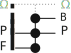
\includegraphics[width=2.5cm]{graphics/development/edit_to_hg_operations/CRE_to_SEC+UNI}
  } \\

  &
  $n_f$ &
  $n_p$ &
  $1$ &
  \pbox{6.0cm}{
    ~\\
    \texttt{SEC} of $B_1$ from $\Omega$ \\
    \texttt{SEC} of $T_p$ from $A_p$, \texttt{INC} of $T_p$ into $B_1$ \\
    \texttt{INC} of $A_f$ into $B_1$
  } &
  \\

  % MERGE
  \midrule
  \multirow{3}{*}{\texttt{MRG} (1)} &
  \multicolumn{4}{p{10cm}}{
    Multiple Areas $A_i$ are unified to $B_1$. The new Area receives a new name distinct from all the names of $A_i$.
  } &
  \multirow{3}{*}{
    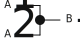
\includegraphics[width=2.5cm]{graphics/development/edit_to_hg_operations/MRG_to_UNI}
  } \\
  &
  $n \geq 2$ &
  $0$ &
  $1$ &
  \pbox{6.0cm}{
    ~\\
    \texttt{UNI} of $\forall A_i$ to $B_1$
  } &
  \\

  \midrule
  \multirow{4}{*}{\texttt{MRG} (2)} &
  \multicolumn{4}{p{10cm}}{
    Multiple Areas $A_i$ are unified, the resulting Area reuses the short and formal name of one of the old Areas ($A_p$) and therefore preserves it. The remaining Areas $A_i$ are incorporated into $A_p$.
  } &
  \multirow{4}{*}{
    \includegraphics[width=2.5cm]{graphics/development/edit_to_hg_operations/MRG_to_INC}
  } \\
  &
  $n \geq 1$ &
  $1$ &
  $1$ &
  \pbox{6.0cm}{
    ~\\
    \texttt{INC} of $\forall A_i$ into $A_p$
  } &
  \\

  \midrule
  \multirow{4}{*}{\texttt{MRG} (3)} &
  \multicolumn{4}{p{10cm}}{
    The same as the previous case, just that $A_p$ receives a new short name and therefore an additional name change is required.
  } &
  \multirow{4}{*}{
    \includegraphics[width=2.5cm]{graphics/development/edit_to_hg_operations/MRG_to_INC+NCH}
  } \\
  &
  $n \geq 1$ &
  $1$ &
  $1$ &
  \pbox{6.0cm}{
    ~\\
    \texttt{INC} of $\forall A_i$ into $A_p$ \\
    \texttt{NCH} of $A_p$
  } &
  \\

  % DISSOLVE

  \midrule
  \multirow{4}{*}{\texttt{DIS} (1)} &
  \multicolumn{4}{p{10cm}}{
    Separate one Area $A_1$ into multiple new Areas $B_i$ and define a territory and name for each of them. Each name is distinct from the name of the old Area.
  } &
  \multirow{4}{*}{
    \includegraphics[width=2.5cm]{graphics/development/edit_to_hg_operations/DIS_to_SEP}
  } \\
  &
  $1$ &
  $0$ &
  $n \geq 2$ &
  \pbox{6.0cm}{
    ~\\
    \texttt{SEP} of $A_1$ into $\forall B_i$
  } &
  \\

  \midrule
  \multirow{5}{*}{\texttt{DIS} (2)} &
  \multicolumn{4}{p{10cm}}{
    Separate multiple Areas $B_1$ from one initial Area $A_p$ and define a territory and name for each of them. One of the separated Areas has the same short and formal name as $A_p$, so it continues its identity and preserves the Area. The remaining new Areas secede from $A_p$.
  } &
  \multirow{5}{*}{
    \includegraphics[width=2.5cm]{graphics/development/edit_to_hg_operations/DIS_to_SEC}
  } \\
  &
  $1$ &
  $1$ &
  $n \geq 1$ &
  \pbox{6.0cm}{
    ~\\
    \texttt{SEC} of $\forall B_i$ from $A_p$
  } &
  \\

  \midrule
  \multirow{4}{*}{\texttt{DIS} (3)} &
  \multicolumn{4}{p{10cm}}{
    The same as the previous case, just that $A_p$ receives a new short name and therefore an additional name change is required.
  } &
  \multirow{4}{*}{
    
\includegraphics[width=2.5cm]{graphics/development/edit_to_hg_operations/DIS_to_SEC+NCH}
  } \\
  &
  $1$ &
  $1$ &
  $n \geq 1$ &
  \pbox{6.0cm}{
    ~\\
    \texttt{SEC} of $\forall B_i$ from $A_p$  \\
    \texttt{NCH} of $A_p$
  } &
  \\

  % CHANGE BORDER

  \midrule
  \multirow{10}{*}{\texttt{CHB} (1)} &
  \multicolumn{4}{p{10cm}}{
    One existing Area $A_1$ is selected and its territory changes. Relative to the old territory some parts of the territory expanded ($T_e$) and some withdrew ($T_w$).
    The part of $T_e$ that expanded into unclaimed land ($T_\Omega \in T_e$) is seceded from $\Omega$ and incorporated into $A_1$.
    The Areas $A_f$ fully covered by $T_e$ are incorporated into $A_1$,
    the Areas $A_p$ partially covered by $T_e$ secede this territory $T_p \in T_e$ to $A_1$.
    $T_w$ will be incorporated into $\Omega$, resulting in unclaimed land.
  } &
  \multirow{10}{*}{
    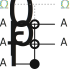
\includegraphics[width=2.5cm]{graphics/development/edit_to_hg_operations/CHB_to_SEC+INC_omega}
  } \\
  &
  $n_f$ &
  $1+n_p$ &
  $0$ &
  \pbox{6.0cm}{
    ~\\
    \texttt{SEC} of $T_\Omega$ from $\Omega$,
    \texttt{INC} of $T_\Omega$ into $A_1$ \\
    \texttt{SEC} of $T_p$ from $A_p$,
    \texttt{INC} of $T_p$ into $B_1$ \\
    \texttt{INC} of $A_f$ into $B_1$ \\
    \texttt{SEC} of $T_w$ from $B_1$,
    \texttt{INC} of $T_w$ into $\Omega$
  } &
  \\

  \midrule
  \multirow{7}{*}{\texttt{CHB} (2)} &
  \multicolumn{4}{p{10cm}}{
    Two existing Areas $A_1$ and $A_2$ are selected and their common border changes. This results in a symmetrical change of territories, made up by two sets of territories: $T_2$ that previously belonged to $A_1$ and is now part of $A_2$ and $T_1$ for which the opposite is true. $T_2$ is seceded by $A_1$ and incorporated into $A_2$, the opposite happenes to $T_1$.
  } &
  \multirow{7}{*}{
    \includegraphics[width=2.5cm]{graphics/development/edit_to_hg_operations/CHB_to_SEC+INC}
  } \\
  &
  $0$ &
  $2$ &
  $0$ &
  \pbox{6.0cm}{
    ~\\
    \texttt{SEC} of $T_2$ from $A_1$,
    \texttt{INC} of $T_2$ into $A_2$ \\
    \texttt{SEC} of $T_1$ from $A_2$,
    \texttt{INC} of $T_1$ into $A_1$
  } &
  \\

  % RENAME

  \midrule
  \multirow{3}{*}{\texttt{REN} (1)} &
  \multicolumn{4}{p{10cm}}{
    One Area $A_1$ is selected and both its short and formal name is changed. Therefore, a new Area $B_1$ is created as a direct successor of $A_1$. This is a special case of a unification with only one Area.
  } &
  \multirow{3}{*}{
    \includegraphics[width=2.5cm]{graphics/development/edit_to_hg_operations/REN_to_UNI}
  } \\
  &
  $1$ &
  $0$ &
  $1$ &
  \pbox{6.0cm}{
    \texttt{UNI} of $A_1$ to $B_1$
  } &
  \\

  \midrule
  \multirow{3}{*}{\texttt{REN} (2)} &
  \multicolumn{4}{p{10cm}}{
    One Area $A_1$ is selected and receives a new short name, but the formal name and therefore the identity is preserved. $A_1$ is updated.
  } &
  \multirow{3}{*}{
    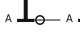
\includegraphics[width=2.5cm]{graphics/development/edit_to_hg_operations/REN_to_NCH}
  } \\
  &
  $0$ &
  $1$ &
  $0$ &
  \pbox{6.0cm}{
    \texttt{NCH} of $A_1$
  } &
  \\

  % CEASE

  \midrule
  \multirow{2}{*}{\texttt{CES} (1)} &
  \multicolumn{4}{p{10cm}}{
    One Area $A_1$ is selected and ceases by incorporating into the universe.
  } &
  \multirow{2}{*}{
    \includegraphics[width=2.5cm]{graphics/development/edit_to_hg_operations/CES_to_INC}
  } \\
  &
  $1$ &
  $0$ &
  $0$ &
  \pbox{6.0cm}{
    \texttt{INC} of $A_1$ into $\Omega$
  } &
  \\

  \bottomrule
\caption{Translation from EditOperations to HG Operations}
\end{longtable}
\label{tab:editoperations_to_hg_operations}
\end{center}
\footnotetext{multiple HG Operations in one row happen exactly at the same time point, so they are combined}

% paragraph reduction_to_hg_operations (end)


% subsection editmode (end)

% ------------------------------------------------------------------------------
\subsection{Design Iterations} % (fold)
\label{sub:design_iterations}

The EditMode is entered throught an edit button on the upper right corner of the user interface.

EditOperation buttons

WorkflowWindow
NewNameTool
NewTerritoryTool
NewHiventBox

% - - - - - - - - - - - - - - - - - - - - - - - - - - - - - - - - - - - - - - -
\paragraph{Paper Prototype} % (fold)
\label{par:paper_prototype}

description of process
image of two prototypes

% paragraph paper_prototype (end)

% - - - - - - - - - - - - - - - - - - - - - - - - - - - - - - - - - - - - - - -
\paragraph{Mockup Prototype} % (fold)
\label{par:mockup_prototype}

description of process
screenshot of two steps in between and of final version

% paragraph mockup_prototype (end)

% - - - - - - - - - - - - - - - - - - - - - - - - - - - - - - - - - - - - - - -
\paragraph{HistoGlobe Interface} % (fold)
\label{par:histoglobe_interface}

screenshot
explanation of all final UI Elements

% paragraph histoglobe_interface (end)

% subsection design_iterations (end)

% section histoglobe_interface (end)


% ==============================================================================
\section{HistoGlobe Application} % (fold)
\label{sec:histoglobe_application}

- the final version of the application behind the interface built on top of the data model

distributed Web-based system
classic approach: UI <-> Client (main program) <-> Server (middleware) <-> DB

% ------------------------------------------------------------------------------
\subsection{System Architecture} % (fold)
\label{sub:system_architecture}


The system developed in this thesis is Web-based. That means, there is a \emph{client}, a Web browser, and a remote Web \emph{server} with a database and a middleware. The Web browser hosts the applications user interface. If the user interacts with a tool the client sends a request to the Web server for new data. The middleware checks the request and queries the necessary data from the database. The data will be transformed and sendt back to the client. On the map and the timeline the new information will be shown.

This clear separation between the data (\emph{model}), the user interface (\emph{view}) and the middleware (\emph{controller}) follows directly from the \emph{model-view-controller pattern}: One part can be changed without interfering the other parts, e.g. if the 2D map is replaced by a 3D globe, only the view changes, but the middleware and the database can stay untouched. Likewise, the implementation of a new database technology has no consequences to the view.

graphic of basic system:
UI
Client-side mechanism
Server-side mechanism
Database

programming languages / Framworks
Client                    HTML
          Less ->         CSS
          CoffeeScript -> JavaScript
Server    Django ->       Python
                          PostgreSQL
                          + PostGIS

% subsection system_architecture (end)

% ------------------------------------------------------------------------------
\subsection{Database Model} % (fold)
\label{sub:database_model}

database model

\begin{compactenum}
  \item The \emph{name} of the Hivent.
  \item A textual \emph{description} of the topic of the Hivent.
  \item The point in time, identified by the Hivent \emph{date}.
  \item The Hivent \emph{location}.
  \item The \emph{historical changes} resulting from the Hivent.
\end{compactenum}


           Hivent
             m
       HistoricalChange
             m
  --------AreaChange------
  |          |           |
  |     ----Area----     |
  m     m          m     m
AreaTerritory      AreaName

no transaction time, only valid / event time
only world time is regarded, not database time.

view

get\_all
save\_operation

% subsection database_model (end)


% ------------------------------------------------------------------------------
\subsection{Computational Model} % (fold)
\label{sub:computational_model}

Class diagram

HistoGlobe

SpatialDisplay -> Map

TimeController  <-> Timeline
                <-> NowMarker

HiventController                AreaController <->  AreasOnMap
HiventHandle                    AreaHandle
Hivent
HistoricalChange    AreaChange  Area
                                AreaName            AreaNameLayerOnMap
                                AreaTerritory       AreaTerritoryLayerOnMap

DatabaseInterface

EditMode -> EditOperation -> EditOperationStep
NewTerritoryTool* NewNameTool NewHiventBox
WorkflowWindow

HistoGraph

LabelManager*

important little utils
  Button, ButtonArea
  NumberInput, TextInput, TextInputArea
  Title
  Watermark
  DoublyLinkedList
  WithinTree
  Geometry -> Polypolygon -> Polygon -> Polyline -> Point

% - - - - - - - - - - - - - - - - - - - - - - - - - - - - - - - - - - - - - - -
translation

EditOperations   CRE   UNI   SEP   TCH   NCH   DES

HG Operations     UNI   INC   SEP   SEC   NCH

% - - - - - - - - - - - - - - - - - - - - - - - - - - - - - - - - - - - - - - -
\paragraph{Functional description} % (fold)
\label{par:functional_description}

Each HG Operation can be described by a mathematical function. The following symbols are used in the equations:

\begin{addmargin}[1em]{0em}
\begin{tabbing}
  symbolxx \= description1xx \= description2 \kill
  $A$ \> set of old Areas that were active before the Historical Change \\
  $B$ \> set of new Areas that are created in the Historical Change \\
  $n:$ \> $n \in \mathbb{N}, n>0$ \> total number of old respectively new Areas \\
  $i:$ \> $i \in [\textbf{1} .. n]$ \> iterator for the current old respectively new Area \\
  $A_0/B_0$ \>    the first old respectively new Area ($i \geq 1 \Rightarrow$ not $A_i/B_i$~!) \\
  $A_i/B_i$ \>    the current old respectively new Area ($i \geq 1 \Rightarrow$ not $A_0/B_0$~!) \\
  $A_i^T/B_i^T$ \>the new territory of the current Area (a polypolygon) \\
  $A_i^N/B_i^N$ \>the new name of the current Area (short and formal name) \\
\end{tabbing}
\end{addmargin}

\vspace{-2.5em}
\begin{align*}
  (B_0)                       &= UNI([A_1 .. A_i .. A_n], B_0^N) \\
  (A_0)                       &= INC(A_0, [A_1 .. A_i .. A_n]) \\
  ([B_1 .. B_i .. B_n])       &= SEP(A_0, [[B_1^T, B_1^N] .. [B_i^T, B_i^N] .. [B_n^T, B_n^N]]) \\
  (A_0, [B_1 .. B_i .. B_n])  &= SEC(A_0, A_0^T, [[B_1^T, B_1^N] .. [B_i^T, B_i^N] .. [B_n^T, B_n^N]]) \\
  (A_0)                       &= NCH(A_0, A_0^N)
\end{align*}

% paragraph functional_description (end)

% - - - - - - - - - - - - - - - - - - - - - - - - - - - - - - - - - - - - - - -
\paragraph{Pseudocode description} % (fold)
\label{par:pseudocode_description}

of the HG operations in an object-oriented manner. The existance of a class \texttt{Area} is assumed. Each \texttt{Area} object has the following member variables: a \texttt{name}, a \texttt{territory} and a list of historical \texttt{predecessors} and \texttt{successors}. Single capital letter variables (\texttt{A}/\texttt{B}) denote arrays of \texttt{Area} objects. Variables with a capital letter followed by a number or lowercase letter (e.g. \texttt{B0}) are single \texttt{Area} objects.

\begin{minipage}[t]{0.47\textwidth}
\begin{lstlisting}[language=pseudocode,
  caption=Unification]
FUNCTION UNI(A, B0_name)
  # create new territory
  B0_territory = NEW Geometry # empty
  FOREACH Ai IN A
    B0_territory.union(Ai.territory)
  # create new area
  B0 = NEW Area(B0_name, B0_territory)
  # establish historical relationships
  FOREACH Ai IN A
    Ai.successors.add(B0)
    B0.predecessors.add(A1)
  # return new area
  RETURN B0
\end{lstlisting}
\end{minipage}    % N.B. the % is very important
\hspace{3.0em}    % N.B. this must go in this line, no blank lines !!!
\begin{minipage}[t]{0.47\textwidth}
\begin{lstlisting}[language=pseudocode,
  caption=Incorporation]
FUNCTION INC(A0, A)
  # update old area with new territory
  temp_terr = NEW Geometry # empty
  FOREACH Ai IN A
    temp_terr.union(Ai.territory)
  A0.territory = temp_terr
  # establish historical relationships
  FOREACH Ai IN A
    Ai.successor.add(A0)
    A0.predecessor.add(A1)
  # return new area
  RETURN A0
\end{lstlisting}
\end{minipage}

\begin{minipage}[t]{0.47\textwidth}
\begin{lstlisting}[language=pseudocode,
  caption=Separation]
FUNCTION SEP(A0, B_data)
  # create each new Area
  B = []
  FOREACH Bi_data in B_data
    B.add(NEW Area(
      Bi_data.name, Bi_data.territory)
    )
  # establish historical relationships
  FOREACH Bi IN B
    A0.successors.add(Bi)
    Bi.predecessors.add(A0)
  # return new areas
  RETURN B

\end{lstlisting}
\end{minipage}    % N.B. the % is very important
\hspace{3.5em}    % N.B. this must go in this line, no blank lines !!!
\begin{minipage}[t]{0.47\textwidth}
\begin{lstlisting}[language=pseudocode,
  caption=Secession]
FUNCTION SEC(A0, A_territory, B_data)
  # update old area with new territory
  A0.territory = A_territory
  # create each new Area
  B = []
  FOREACH Bi_data in B_data
    B.add(NEW Area(
      Bi_data.name, Bi_data.territory)
    )
  # establish historical relationships
  FOREACH Bi IN B
    A0.successors.add(Bi)
    Bi.predecessors.add(A0)
  # return old and new areas
  RETURN [A0, B]

\end{lstlisting}
\end{minipage}

\vspace{-1.5em}
\begin{minipage}[t]{0.47\textwidth}
\begin{lstlisting}[language=pseudocode,
  caption=Name Change]
FUNCTION NCH(A0, A_name)
  # update old area with new name
  A0.name = A_name
  # return updated area
  RETURN A0

\end{lstlisting}
\end{minipage}

% paragraph pseudocode_description (end)


\paragraph{Execute Historical Change} % (fold)
\label{par:execute_historical_change}

execute function for all operations the same

% - - - - - - - - - - - - - - - - - - - - - - - - - - - - - - - - - - - - - - -
\begin{lstlisting}[language=pseudocode,
  caption=class HGOperation]
## member variables
old_areas = []          # Area
new_areas = []          # Area
update_name = {
  area :          null  # Area
  old_name :      null  # AreaName
  new_name :      null  # AreaName
}
update_territory = {
  area :          null  # Area
  old_territory : null  # AreaTerritory
  new_territory : null  # AreaTerritory
}

## main function
FUNCTION execute(direction)

  # hide old areas
  FOREACH old_area IN old_areas
    IF direction IS 1 # forward change
      old_area.hide()
    ELSE              # backward change
      old_area.show()

  # show new areas
  FOREACH new_area IN new_areas
    IF direction IS 1 # forward change
      new_area.show()
    ELSE              # backward change
      new_area.hide()

  # check if the area name is updated
  IF update_name.area
    IF direction IS 1 # forward change
      update_name.area.name = new_name
    ELSE              # backward change
      update_name.area.name = old_name
    update_name.area.update()

  # check if the area territory is updated
  IF update_territory.area
    IF direction IS 1 # forward change
      update_territory.area.territory = new_territory
    ELSE              # backward change
      update_territory.area.territory = old_territory

\end{lstlisting}

% paragraph execute_historical_change (end)

HistoGraph
\begin{lstlisting}[language=pseudocode,
  caption=plotting Areas on the HistoGraph,
  label=lst:histograph_plot]
FUNCTION plot(reference_area, plot_start_date, plot_end_date)
  # plot the current Area
  # logic is omitted

  # recursively plot in historically backward direction
  FOREACH predecessor IN reference_area.predecessors
    IF predecessor.end_date >= plot_start_date
      plot(predecessor)

  # recursively plot in historically forward direction
  FOREACH successor IN reference_area.successors
    IF successor.start_date <= plot_end_date
      plot(successor)
\end{lstlisting}

store Hivents in DoublyLinkedList

% \begin{figure}[ht]
%   \centering
%   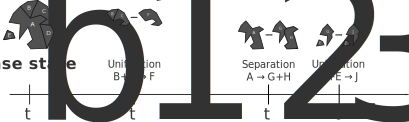
\includegraphics[width=0.8\textwidth]{graphics/basics/stdm/event-based_spatio-temporal_data_model}
%   \caption{The Event-Based Spatio-Temporal Data Model}
%   \label{fig:event-based_spatio-temporal_data_model}


A main problem is to maintain the integrity of the spatial topology when a new change gets inserted not at the end of the list. A simple example shows that problem: Given geo-object $X$ is part of the inital base configuration at change $t_b$. At a later change, e.g. $t_y$ $X$ gets replaced by object $Y$. If a new change that updates $X$ to $X'$ gets inserted before at time point $t_x < t_y$, then $t_y$ is not integer anymore, because object $X$ does not exist. That is why on insertion of a change, all succeeding changes have to be tested for integrity and it might be necessary to update later changes.


% subsection computational_model (end)

% section histoglobe_application (end)

% chapter development (end)

% ==============================================================================

\vspace{2em}
transition to next chapter